\section{Kleine Lawinenkunde}

Das Lawinenbulletin ist eine \textbf{Prognose der Lawinengefahr} für eine geografische Region und \textbf{nicht für den Einzelhang}.

Die Hauptausgabe des Lawinenbulletin erscheint um 17 Uhr auf der Website des SLF \href{https://www.slf.ch}{www.slf.ch} und in der App \enquote{White Risk}.
Je nach Situation erscheint morgens um 8 Uhr eine weitere Ausgabe.

Die Lawinengefahr wird mit der \textit{Gefahrenstufe} inklusive \textit{Geltungsbereich} und den typischen \textit{Lawinenproblemen} angegeben.

\begin{center}
  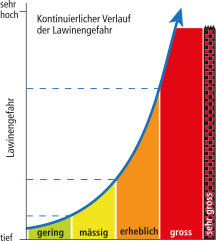
\includegraphics[width=0.82\linewidth]{bulletin.svg.pdf}
\end{center}

Die \textbf{Gefahrenstufen} gibt uns eine erste Einschätzung über die prognostizierte Lawinensituation in der Region.

\newcolumn

Folgende Gefahrenstufen sind definiert:

\begin{enumerate}
  \item{
    \textbf{Gering} -- günstige Situation
    \begin{itemize}
      \item{Es sind keine Alarmzeichen feststellbar.}
      \item{Extrem steile Hänge einzeln befahren.}
      \item{Absturzgefahr beachten.}
      \item{Für etwa 20\% des Winters prognostiziert.}
      \item{Rund 5\% aller Todesopfer.}
    \end{itemize}
  }
  \item{
    \textbf{Mässig} -- mehrheitlich günstige Situation
    \begin{itemize}
      \item{Vereinzelt sind Alarmzeichen feststellbar.}
      \item{Vorsichtige Routenwahl, vor allem im angegebenen Geltungsbereich des Bulletin.}
      \item{Für etwa 50\% des Winters prognostiziert.}
      \item{Rund 30\% aller Todesopfer.}
    \end{itemize}
  }
  \item{
    \textbf{Erheblich} -- kritische Situation
    \begin{itemize}
      \item{Wummgeräusche und Risse sind typisch.}
      \item{Defensive Routenwahl ist empfohlen.}
      \item{Sehr steile Hänge meiden.}
      \item{Unerfahrenen wird empfohlen zu verzichten.}
      \item{Für etwa 30\% des Winters prognostiziert.}
      \item{Rund 50\% aller Todesopfer.}
    \end{itemize}
  }
  \item{
    \textbf{Gross} -- sehr kritische Situation
    \begin{itemize}
      \item{Spontane Lawinen sind wahrscheinlich.}
      \item{Auf mässig steiles Gelände beschränken.}
      \item{Unerfahrenen wird empfohlen zu verzichten.}
      \item{Für wenige Tage im Winter prognostiziert.}
      \item{Rund 10\% aller Todesopfer.}
    \end{itemize}
  }
  \item{
    \textbf{Sehr Gross} -- ausserordentliche Situation
    \begin{itemize}
      \item{Sehr grosse Lawinen sind zu erwarten.}
      \item{Strassen und Dörfer in Tallage sind gefährdet.}
      \item{Verzicht auf Schneesport abseits geöffneter Abfahrten und Routen wird empfohlen.}
      \item{Wird sehr selten prognostiziert.}
      \item{Rund 1\% aller Todesopfer.}
    \end{itemize}
  }
\end{enumerate}

\newcolumn

Bei einem trockenen Lawinenproblem wird zudem eine Zwischenstufe mittels Minus ($-$) Gleich ($=$) oder Plus ($+$) angegeben.

\textit{Das bedeutet nicht, dass wir bei einem 3$-$ mehr riskieren dürfen. Für die Entscheidung ausschlaggebend ist immer die Hauptstufe.}

\begin{center}
  
\includegraphics[width=0.8\linewidth]{gefahrenplot.svg.pdf}
\end{center}

Der \textbf{Geltungsbereich} beschreibt \textit{wo} -- und gegebenenfalls \textit{wann} -- die Gefahrenstufe gilt.
Dies umfasst folgende Informationen:

\begin{itemize}
  \item{\textbf{Höhenlage} -- In welcher Höhe gilt die Gefahrenstufe. Hier wird entweder eine minimale oder maximale Höhe angegeben.}
  \item{\textbf{Exposition} -- Für welche Hanglage gilt die Gefahrenstufe. Hier wird ein Abschnitt auf der Kompassrose angegeben.}
  \item{\textbf{Tageszeit} -- Ab welcher Tageszeit gilt die Gefahrenstufe. Wird nur genannt, wenn sich die Gefahrenstufe im Tagesgang markant ändert.}
\end{itemize}

Das typische \textbf{Lawinenproblemen} schliesslich beschreibt die Schneeschicht, von der bei der genannten Gefahrenstufe und im Geltungsbereich die Hauptgefahr ausgeht.
Dies umfasst folgende Situationen:

\begin{itemize}
  \item{
    \textbf{Altschnee} -- bei einer Schwachschicht
    \begin{itemize}
      \item{Physikalische Prozesse auf und in der Schneedecke verändern deren Struktur und Stabilität.}
      \item{Wummgeräusche sind ein Alarmzeichen}
      \item{Lawinen können auch bei mässiger Lawinengefahr gefährlich gross werden!}
      \item{Gefahr droht vor allem dort, wo die Schwachschicht nahe an der Oberfläche ist.}
    \end{itemize}
  }
  \item{
    \textbf{Neuschnee} -- bei frisch gefallenem Schnee
    \begin{itemize}
      \item{Kann als Schneebrettlawine abgleiten}
      \item{Frische Schneebrettlawinen sind ein Hinweis}
      \item{Verbreitung der Gefahrenstellen meist flächig}
      \item{In der Höhe oft kritischer}
    \end{itemize}
  }
  \item{
    \textbf{Triebschnee} -- von Wind verfrachtetem Schnee
    \begin{itemize}
      \item{Frischer Triebschnee ist oft sehr auslösefreudig}
      \item{Kann als Schneebrettlawine abgleiten}
      \item{Rissbildung und frische Schneebrettlawinen können auf die Gefahr hinweisen}
      \item{Sastrugi, Wechten und Dünen sind Anzeichen dafür, dass der Wind gewütet hat}
      \item{Triebschnee sammelt sich im Windschatten.}
    \end{itemize}
  }
  \item{
    \textbf{Nassschnee} -- bei Wärme und/oder Regen
    \begin{itemize}
      \item{Nasse Lawinen können spontan und auch bei einer Hangneigung unter 30° abgehen.}
      \item{Im Frühling wird oft im Tagesgang ein Nassschnee Problem prognostiziert.}
      \item{Ein früher Start und eine frühzeitige Rückkehr ist empfohlen.}
      \item{Bei einer Warmwetterphase oder ungenügender Abstrahlung Abkühlung abwarten.}
    \end{itemize}
  }
  \item{
    \textbf{Gleitschnee} -- bei Rissen (sog. Fischmäuler)
    \begin{itemize}
      \item{Oft auf glattem Untergrund und stark besonnten Hängen.}
      \item{Die Gefährdung durch Gleitschnee ist meist von untergeordneter Bedeutung.}
      \item{Gleitschneelawinen können \textit{nicht} durch eine Person ausgelöst werden.}
      \item{Bereiche unterhalb von Gleitschneerissen sollten gemieden oder zügig passiert werden.}
    \end{itemize}
  }
\end{itemize}

\newcolumn

Für trockene Lawinen gibt es ein nützliches Hilfsmittel: Die grafische Reduktionsmethode.
Die grafische Reduktionsmethode bietet eine grobe Beurteilung der Lawinenauslösewahrscheinlichkeit.

\begin{center}
  \includegraphics[width=0.95\linewidth]{risikomatrix.svg.pdf}
\end{center}

\newcolumn